\documentclass{IIBproject}

\usepackage{setspace}

\usepackage{amssymb,amsmath,amsthm}
\usepackage{units}
\usepackage{cite}
\usepackage{subfigure}
\usepackage{minted}
\usepackage{url}
\usepackage[margin=2.5cm]{geometry}
\usepackage{multirow}

\usepackage[retainorgcmds]{IEEEtrantools}

% required to get proper length monospace underscores
\usepackage[T1]{fontenc}

\DeclareMathOperator*{\argmax}{arg\,max}
\DeclareMathOperator*{\argmin}{arg\,min}

\usepackage{graphicx,ctable,booktabs}

\pagestyle{empty}
\onehalfspacing

\begin{document}

% Title Page
\author{Rodrigo Queiro (DOW)}
\title{Machine Learning for Control}
\projectgroup{F}
\maketitle
\thispagestyle{empty}

% Summary
\renewcommand{\abstractname}{Technical Abstract}
\begin{abstract}
  technical abstract\ldots
\end{abstract}
\pagestyle{plain}
\tableofcontents
\newpage

\section{Introduction}

Balancing a unicycle is a very challenging task for a
human rider. Many attempts have been made to achieve this task, using a
variety of models for the action of the rider. Some represent the rider as a
flywheel or pendulum in the coronal plane, allowing direct compensation of
falling to the side\cite{ref:zenkov,ref:murata}, as in
Figure~\ref{fig:murata}. Other use a more realistic (and challenging) model of
a flywheel in the horizontal plane\cite{ref:vos,ref:naveh}, as in
Figures~\ref{fig:naveh_unicycle}, but none of these
have reliably balanced a real unicycle.

\begin{figure}[htbp]
  \begin{center}
    \subfigure[Murata Girl]{
      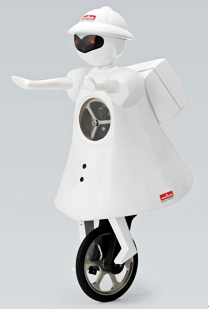
\includegraphics[height=5cm]{figures/murata_girl.jpg}
      \label{fig:murata}
    }
    \subfigure[Naveh's Model]{
      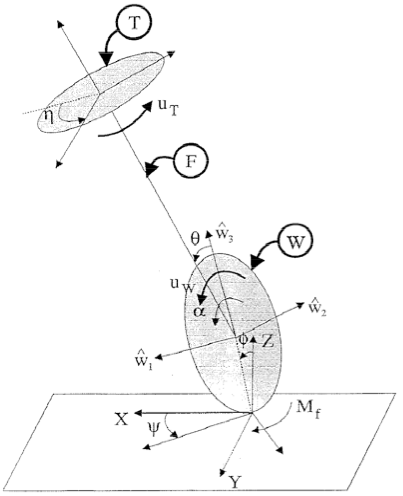
\includegraphics[height=5cm]{figures/naveh_unicycle.png}
      \label{fig:naveh_unicycle}
    }
    \subfigure[2D Problem]{
      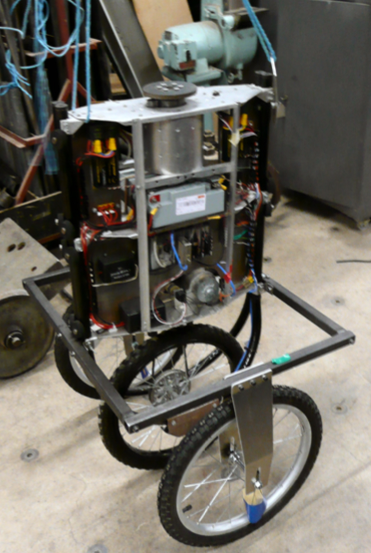
\includegraphics[height=5cm]{figures/forster_unicycle.png}
      \label{fig:forster_unicycle}
    }
    \subfigure[3D Problem]{
      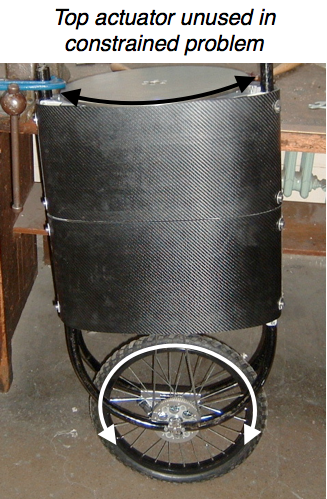
\includegraphics[height=5cm]{figures/3d_unicycle.png}
      \label{fig:3d_unicycle}
    }
    \end{center}
    \caption{Different balance problems}
    \label{fig:unicycles}
    \end{figure}

In 2004/2005 Mellors and Lamb \cite{ref:mellors,ref:lamb} built a robotic
unicycle, shown in Figure~\ref{fig:3d_unicycle}, intending to design a controller to balance it. However, they were
only able to complete the construction of the unicycle. In 2007/2008,
D'Souza-Mathew resumed work, replacing a wheel sensor and attempting to design
a controller. He simplified the problem by removing the ability to fall to the
side, reducing it to 2D dynamic control: the inverted pendulum (from
now on referred to as the 2D system). This is shown in
Figure~\ref{fig:forster_unicycle}. He was unable to balance the unicycle due to
hardware problems.

Next, in 2008/2009 Forster analysed the dynamics of both the 2D problem and
the unrestricted 3D unicycle\cite{ref:forster}. Again, hardware problems
prevented him from balancing the 2D system, and although he designed a
controller for the 3D unicycle, it was not even tested in simulation. Given
the simplicity of his approach compared to those of Vos and Naveh
\cite{ref:vos,ref:naveh}, it appears unlikely to work.

One thing all these approaches have in common is that their first step is a
series of simplifying assumptions about the dynamic system. They ignore the
non-linearities like motor dead-zones and wheel friction that are present in
any real-world system, and attempt to design a controller to stabilise the
idealised system. In many cases, this approach is very successful. However,
D'Souza-Mathew and Forster found that their model was invalid since the
unicycle's motor drive didn't react faster enough. Vos and Naveh had to use
complex, approximate techniques to model the unicycle.

An alternative ``intelligent'' approach to control involves learning the
dynamics of the system directly, instead of relying on assumptions and
mechanical analysis. Various methods for this have been used, but many require
prohibitively large amounts of data from the system. One method due to
Rasmussen and Deisenroth, known here as Reinforced Model Learnt Control
(RMLC), achieves unprecedented data efficiency, and has been successfully used
to stabilise a computer simulation of a 3D
unicycle\cite{ref:rasdei08,ref:rasdei11}.

In 2009/2010, McHutchon successfully applied RMLC to the 2D system
\cite{ref:mchutchon}. However, since he had to make significant changes to the
unicycle hardware and software to achieve this, he did not have time to
attempt to balance the 3D unicycle.

The principle objective of this project is to apply RMLC to the unrestricted
3D unicycle. This includes the solution of problems identified by McHutchon,
as well as other problems identified during the project.


\section{Reinforced Model Learnt Control}

\begin{figure}[htbp]
  \begin{center}
    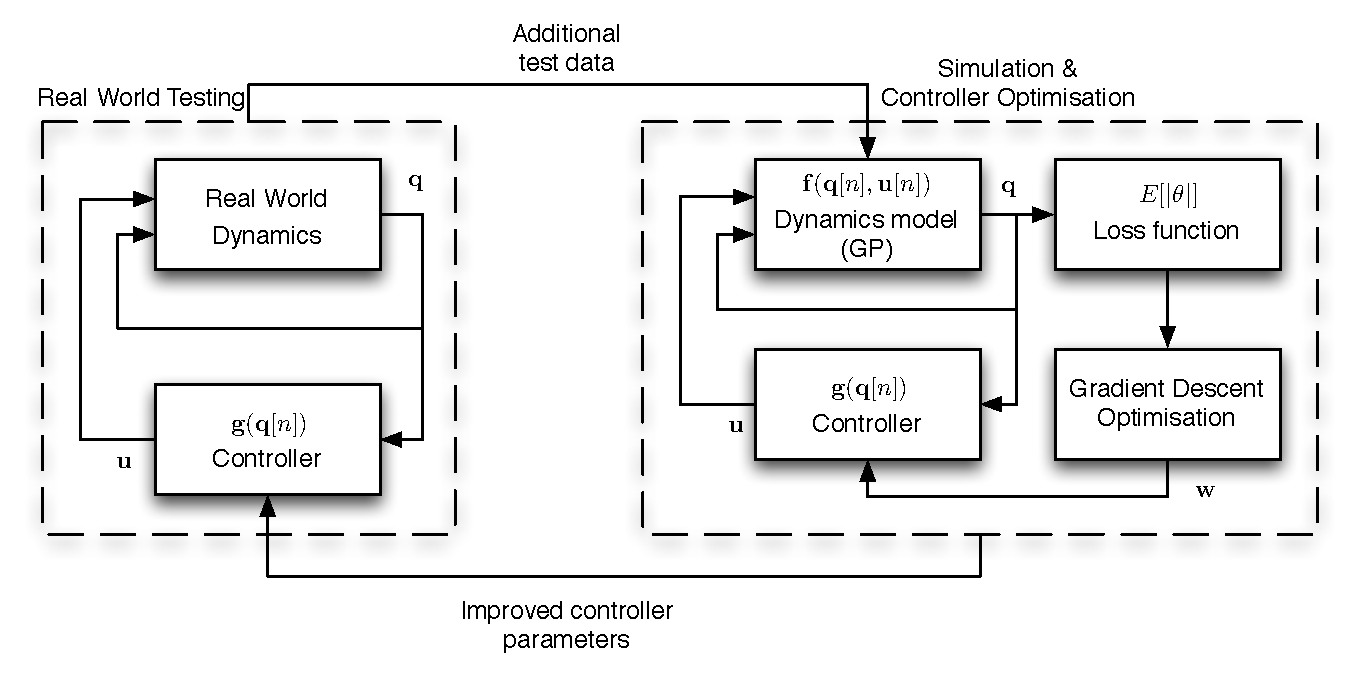
\includegraphics[width=14cm]{figures/GPRMLC.pdf}
    \end{center}
    \caption{Reinforced Model Learnt Control}
    \label{fig:rmlc_flowchart}
    \end{figure}

The main technique in this project is Reinforced Model Learnt Control,
diagrammed in Figure~\ref{fig:rmlc_flowchart}. At its core, it assumes that
the system (in this case, the unicycle) can be modelled in discrete time as:
\[
  \boldsymbol{q}[n+1] = \boldsymbol{f}(\boldsymbol{q}[n],
  \boldsymbol{u}[n])
\]

In this equation, $\boldsymbol{q}[n]$ is the state of the system at time $n$,
and $\boldsymbol{u}[n]$ is control input at time $n$. In the case of the
unicycle, $\boldsymbol{q}$ consists of angles and angular velocities of the
components of the unicycle, and the position of the unicycle.
$\boldsymbol{u}$ consists of the commands sent to the wheel and flywheel
motors.

This function, $\boldsymbol{f}$, is modelled as a Gaussian Process (GP). By
using Gaussian Process Regression (GPR), we can estimate any continuous
function from sampled inputs and outputs. For a description of the mechanics
of GPR, refer to \cite{ref:gpml}. When the unicycle runs, we get
a series of states and control inputs that can be converted to samples of
$\boldsymbol{f}$, and this allows us to use GPR to estimate
$\boldsymbol{f}$ at any point. This estimated $\boldsymbol{f}$ is referred to
as the \textbf{dynamics model}.

By successively applying $\boldsymbol{f}$ to an initial distribution of
possible starting states, we can estimate, with confidence bounds, a
distribution of states over some finite horizon. This is referred to as
\textbf{simulation} of the system. Then, a \textbf{loss function} is applied
to the state distributions---this might find, for example, the expected
distance between the top of the unicycle and the upright position.  Summing
these losses over the horizon gives a numerical score that rates how well the
dynamics model believes a given controller will balance the unicycle. This
loss score penalises uncertainty as well as falling.

The gradient of the loss with respect to the controller parameters can be
calculated, and this allows standard gradient descent optimisation methods to
be used to find a locally optimal controller (for the estimated dynamics
model). This process is shown as the right-hand box, ``Simulation \&
Controller Optimisation'', in Figure~\ref{fig:rmlc_flowchart}, and is referred
to as \textbf{training} a controller.

Once a optimal controller has been trained on the simulated system, a
\textbf{rollout} is performed on the real system (``Real World Testing'' in
Figure~\ref{fig:rmlc_flowchart}). This generates a log of states and control
inputs, which can be converted into more samples of $\boldsymbol{f}$,
improving the quality of the dynamics model and allowing a better controller
to be trained. This process is repeated iteratively until the dynamics model
is sufficiently accurate that the trained controllers perform well on the real
system.

\subsection{Practical Concerns}

There are many different decisions to make when implementing the RMLC
strategy, which are detailed in this section. Fortunately, due to previous
work on stabilising both the real 2D system and the simulation of the 3D
unicycle, we had a lot of information on which choices can work well in these
situations, and which are most important.

\subsubsection{GPR Implementation}
The GPR system has many configurable parameters, but fortunately the form used
previously had proven very robust. This project uses a zero-mean GP with a
squared exponential covariance function, with automatic relevance detection.
This has the form:
\[
  k(\boldsymbol{x}, \boldsymbol{x}') = \alpha^2 \exp \left(\sum_{d=1}^D -
  \frac{(x_d-x_d')^2}{2 l_d^2}\right)
\]

This expression contains hyperparameters for the signal variance $\alpha^2$
and the length scales $l_d$. An additional hyperparameter involved in the
regression is the noise variance, $\sigma_\varepsilon^2$. These parameters are
chosen to best fit the data without overfitting with the maximum likelihood
(ML) method\cite{ref:gpml}. The optimal values of these hyperparameters are
very useful for interpreting how accurate the dynamics model is: a high SNR
$\frac{\alpha}{\sigma_\varepsilon}$ suggests the model can predict very
well.  Furthermore, automatic relevance detection is provided by the length
scales - if a variable is not useful for predicting, the ML length scale will
tend to $\inf$.

\subsubsection{Choice of State Vector}

The state vector $\boldsymbol{q}[n]$ should be chosen to ensure that the
future states are a function only of the current state, and current and future
control inputs. In other words, the states should form a Markov Chain:
\[
  P(\boldsymbol{q}[n+1] | \boldsymbol{q}[i]\textrm{ for } i = 1, \dots, n)
  = P(\boldsymbol{q}[n+1] | \boldsymbol{q}[n])
\]

Forster's analysis suggested the following state to be suitable, which was
found by Rasmussen to be sufficient to model the simulation of the 3D
unicycle.

\[
\boldsymbol{q}[n] = \left[ \begin{array}{ll}
  \dot{\theta} & \textrm{roll angular velocity} \\
  \dot{\phi} & \textrm{yaw angular velocity} \\
  \dot{\psi}_w & \textrm{wheel angular velocity} \\
  \dot{\psi}_f & \textrm{pitch angular velocity} \\
  \dot{\psi}_t & \textrm{flywheel (turntable) angular velocity} \\
  x_c & \multirow{2}{*}{\textrm{position of target in unicycle's reference
  frame}} \\
  y_c & \\
  \theta & \textrm{roll angle} \\
  \psi_f & \textrm{pitch angle} \\
\end{array}\right]
\]

\begin{figure}[htbp]
  \begin{center}
    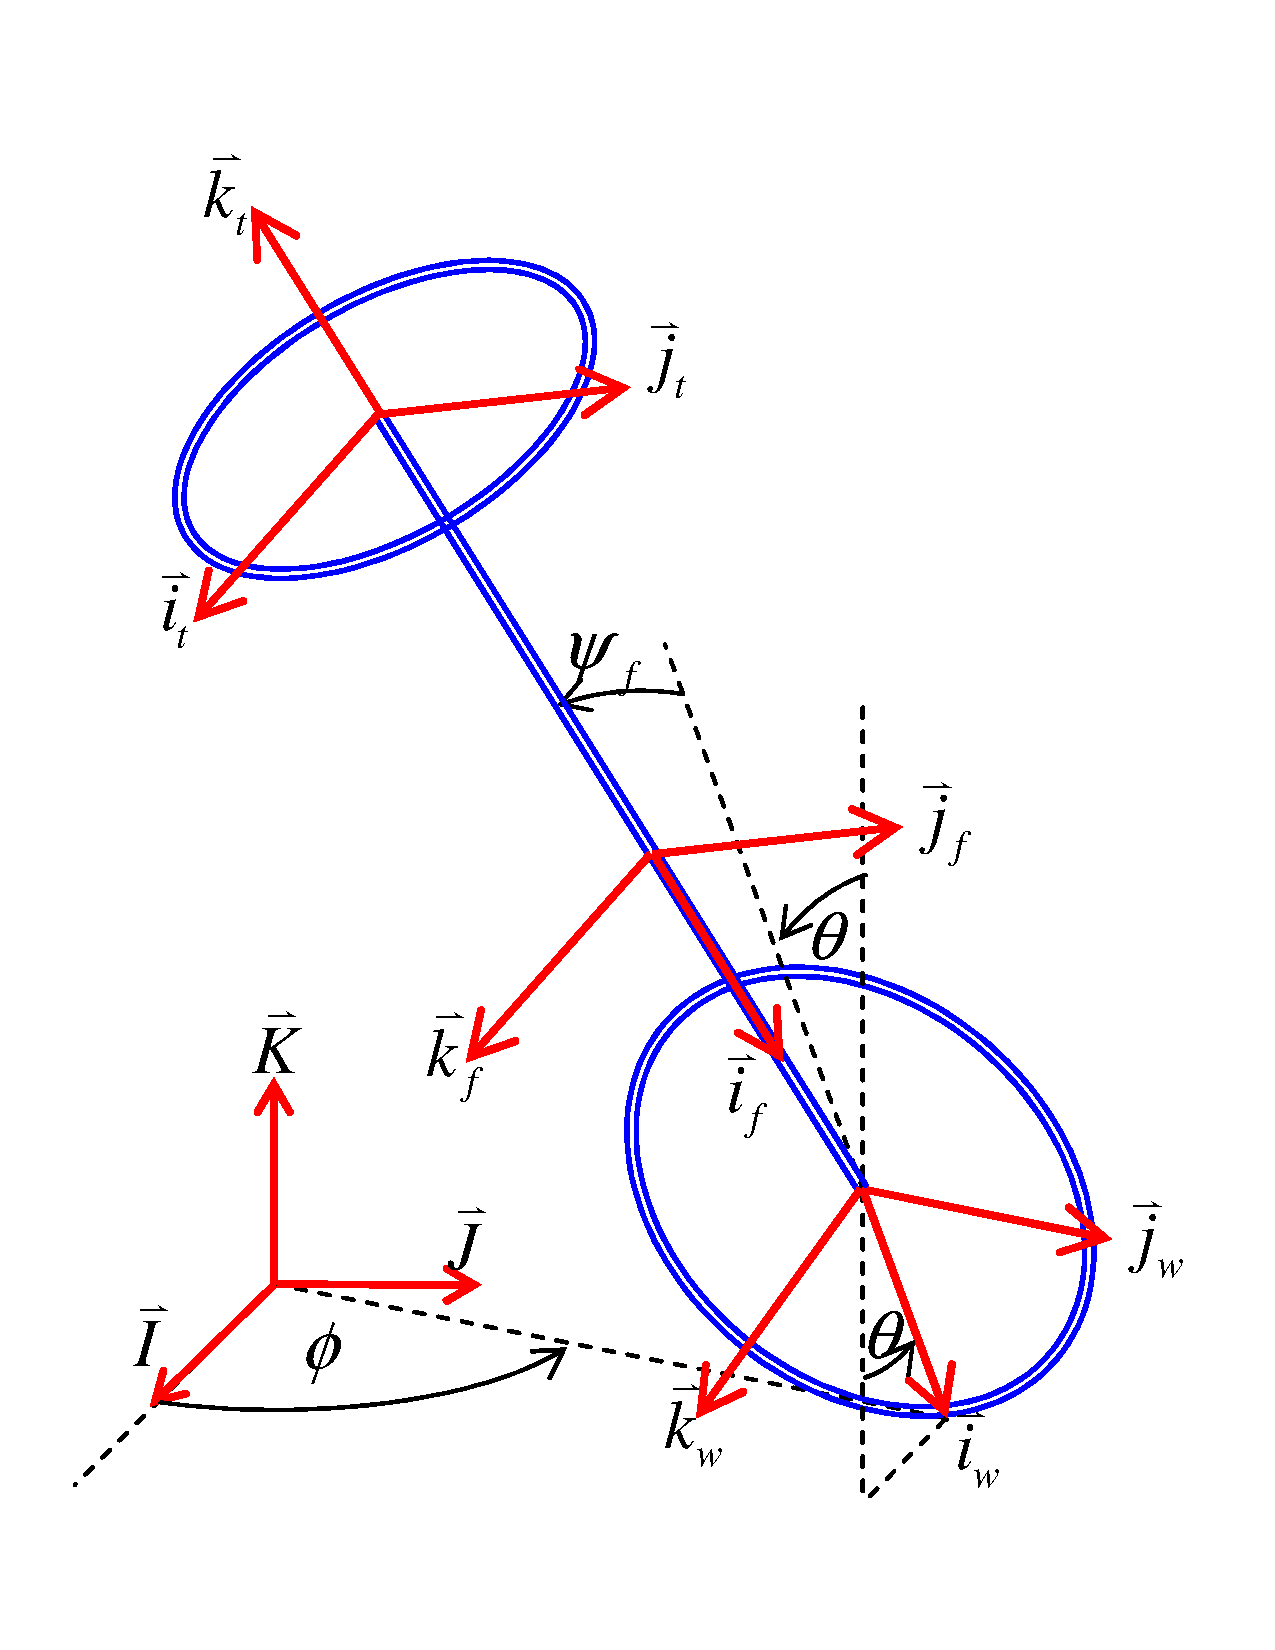
\includegraphics[height=8cm]{figures/angles.pdf}
    \end{center}
    \caption{Diagram showing Euler angles for the rotation of the unicycle
    (from \cite{ref:forster})}
    \label{fig:unicycle_angles}
    \end{figure}

However, this ignores the presence of unobserved states in the system like
delays, backlash in the gears, etc. To help the dynamics model deal with these
problems, we tried giving it access to the previous state and control input,
in effect modelling it as a 2$^\textrm{nd}$ order Markov chain:
\[
  \boldsymbol{q}_2[n] = \left[ \begin{array}{l}
    \boldsymbol{q}[n-1] \\
    \boldsymbol{u}[n-1] \\
    \boldsymbol{q}[n] \\
  \end{array} \right]
\]

This significantly improved the accuracy of the dynamics model, which in turn
suggests that unobserved states are significant in the behaviour of the real
unicycle. 

\subsubsection{Controller Form}

The most basic form of controller is a linear controller,
$\boldsymbol{g}(\boldsymbol{q}[n]) = \boldsymbol{W} \boldsymbol{q}[n] +
\boldsymbol{p}$, where $\boldsymbol{W}$ is a matrix of weights and
$\boldsymbol{p}$ is a vector of offsets. This form is capable of stabilising
the ideal inverted pendulum, and indeed proved sufficient to stabilise the 2D
system.

However, the linear controller cannot generate the correct turning command as
shown in Figure~\ref{fig:xor}---this is equivalent to the XOR problem, and can
be solved by using a quadratic controller. This takes the form:
\[
  g_i(\boldsymbol{q}[n]) = p_i + \sum_{j=1}^D w_{i,j} q_j[n] +
    \sum_{j=1}^D \sum_{k=j}^D h_{i,j,k} q_j[n] q_k[n]
\]
  
\begin{figure}[htbp]
  \begin{center}
    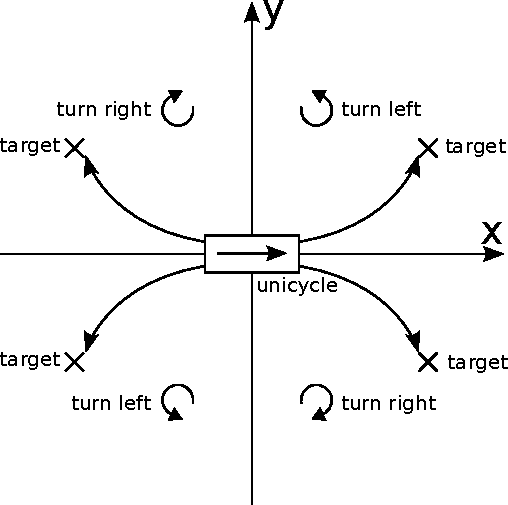
\includegraphics[width=8cm]{figures/xor.pdf}
    \end{center}
    \caption{Correct turning command in unicycle-centred coordinates}
    \label{fig:xor}
    \end{figure}

It was found that the controllers performed significantly better when using
$\boldsymbol{q}_2[n]$ as input, instead of $\boldsymbol{q}[n]$. To understand
this, consider the effect with a linear policy: the controller for the
augmented state is equivalent to a combination of a two-tap FIR filter and a
first-order IIR filter on the original state:
\begin{IEEEeqnarray*}{rCl}
  \boldsymbol{u}[n] &=& 
  \boldsymbol{g}(\boldsymbol{q}_2[n]) = \boldsymbol{W} \boldsymbol{q}_2[n] \\
   &=& \boldsymbol{W}_1 \boldsymbol{q}[n-1] + \boldsymbol{W}_2
   \boldsymbol{u}[n-1] + \boldsymbol{W}_3 \boldsymbol{q}[n]
  \end{IEEEeqnarray*}

This allows the RMLC system to create basic low or high-pass filters in
the controller, and this additional freedom improved the subjective quality of
the controllers trained.

\begin{itemize}
  \item GPR implementation (choice of covariance function, sparse
    approximations, etc.)
  \item contents of the state vector
  \item form of the controller (e.g. linear:
    $\boldsymbol{g}(\boldsymbol{q}[n]) =
    \boldsymbol{w}^\textrm{T}\boldsymbol{q}[n]$)
  \item loss function
  \item timestep for conversion to discrete time
    \end{itemize}

\section{Apparatus and Experimental Results}

\section{Results and Discussion}

\section{Conclusions}

\bibliography{iibproject}
\bibliographystyle{unsrt}

\pagebreak
\appendix

\section{Extra Stuff}

\end{document}
